\section{Part 2}

\subsection{Schematic}
\begin{figure}[H]
\centering
	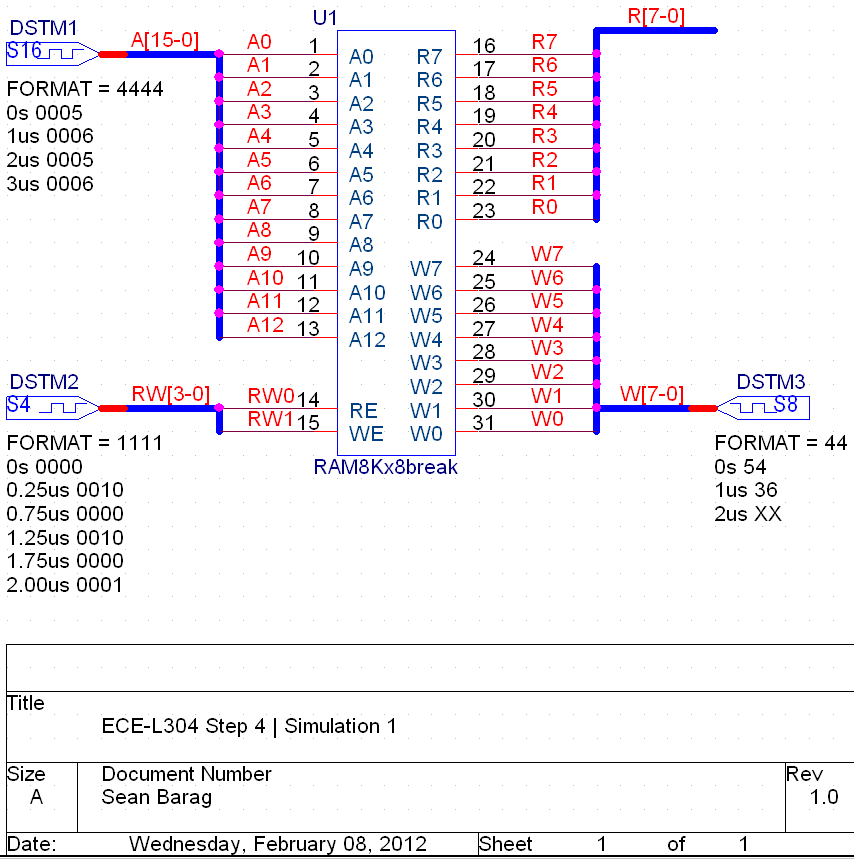
\includegraphics[width=.8\textwidth]{img/shot/schem1.png}
	\parbox{.8\textwidth}{
	\caption[Part 2 Schematic]{PSpice schematic for the circuit simulated in
	part two of step four.}
	\label{f:schem2}}
\end{figure}

\subsection{Simulation}
\begin{figure}[H]
\centering
	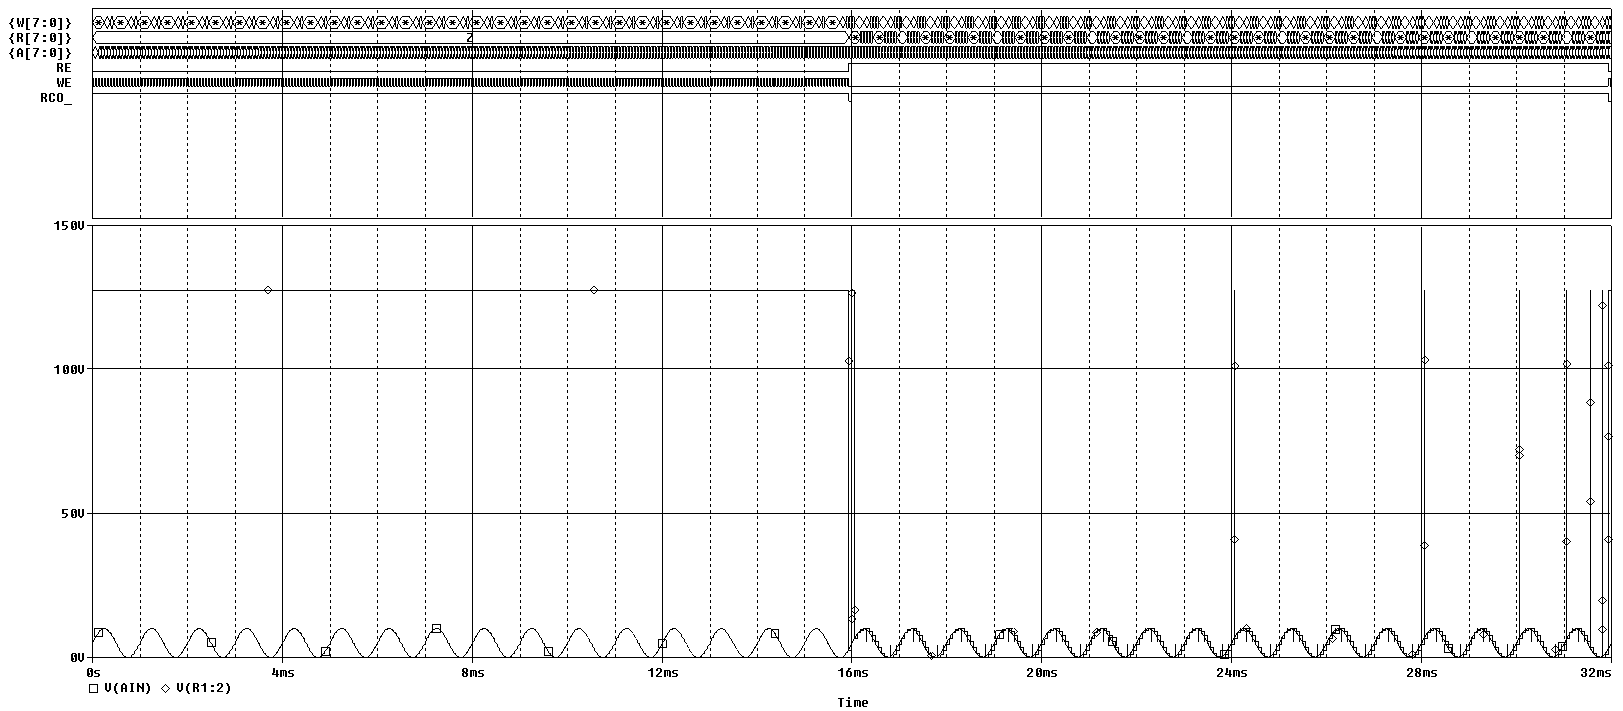
\includegraphics[width=.8\textwidth]{img/shot/sim2_plot1.png}
	\parbox{.8\textwidth}{
	\caption[Part 2 Simulation Results 1]{Results of simulating the schematic
	shown in Figure~\ref{f:schem2} for one full read-write cycle (in this
	case~\SI{32}{\milli\second}) with a~\SI{256}{\volt} supply.  A larger
	version of this figure is available in appendix
	Figure~\ref{f:schem2plot1_big}.}
	\label{f:schem2plot1}}
\end{figure}

\begin{figure}[H]
\centering
	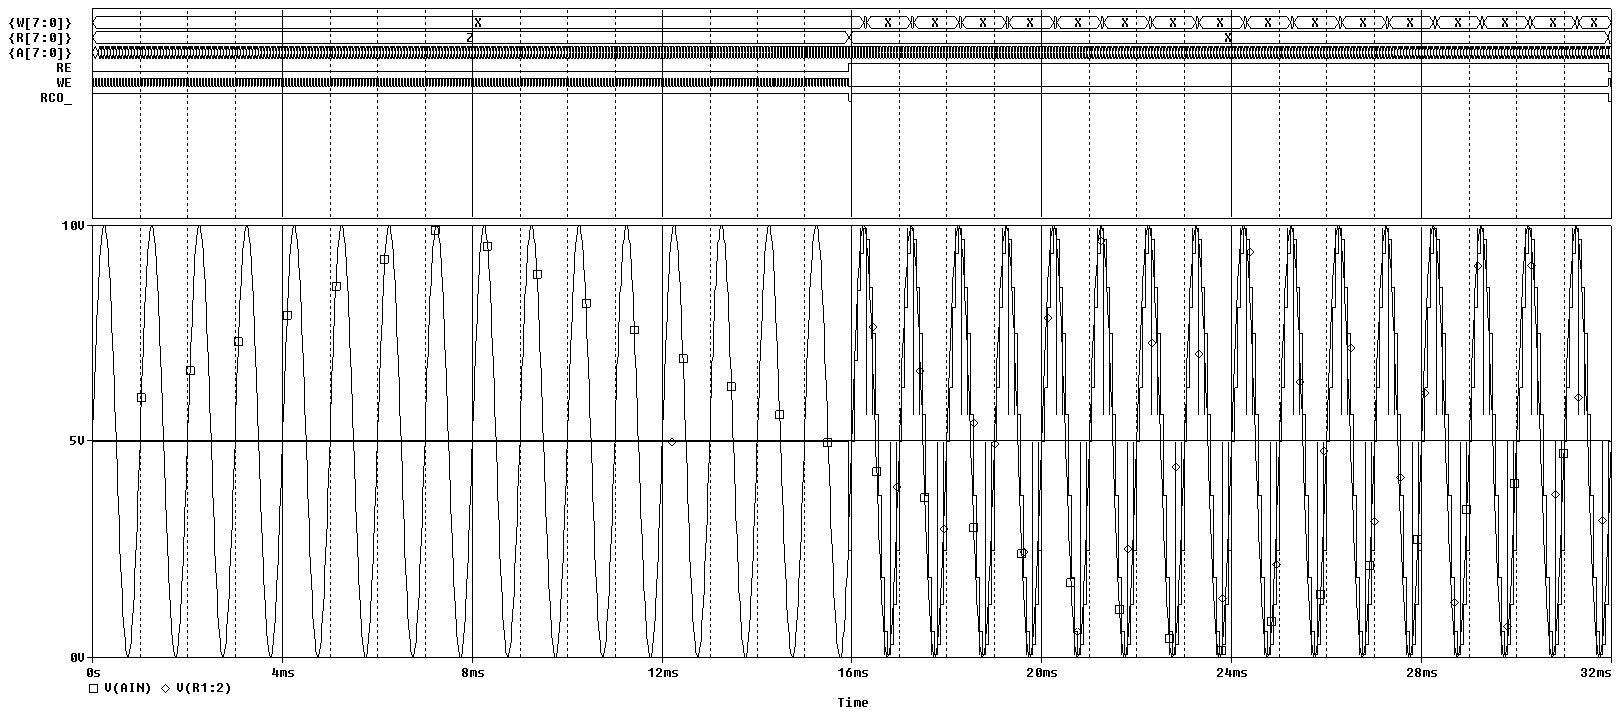
\includegraphics[width=.8\textwidth]{img/shot/sim2_plot2.png}
	\parbox{.8\textwidth}{
	\caption[Part 2 Simulation Results 2]{Results of simulating the schematic
	shown in Figure~\ref{f:schem2} for one full read-write cycle (in this
	case~\SI{32}{\milli\second}) for a supply voltage of~\SI{10}{\volt}.  A
	larger version of this figure is available in appendix
	Figure~\ref{f:schem2plot2_big}.}
	\label{f:schem2plot2}}
\end{figure}

\subsection{Results}
